\section{実験方法}
収穫物の特性を計測する手順は以下のとおりである.
計測する特性は3.1節で提案した特性と, アプローチ面積を求めるために花柄と果実の幅をそれぞれ計測する.
計測対象は30個のピーマンだが, 奥の方にあってスキャンできていないものや, 3Dモデルが大きく欠損していて計測が難しいものは計測結果からは除外する.

\begin{enumerate}
  \item 左から順に人が視認できるピーマン30個にID付け用のシールを貼る
  \item シールを貼ったピーマンがあるピーマン株に対して, Artec Leoを用いて3Dスキャンを行う
  \item 計測して得たピーマン株の3DモデルをBlender内に取り込み, 特性を計測する
\end{enumerate}

計測の例を \figref{Fig:measurement1} \verb|〜| \figref{Fig:measurement3} に示す. 
ピーマン株が複雑であることや, 3Dモデルが一部欠損している場合があり, 特性の計測を自動化することが困難だったため, 今回は手動で行った.
各障害物間距離は, 花柄と果実の内部を含まず, 花柄または果実の中心から障害物までの最小距離と思われる部分を計測した.

\vspace{5mm}
\begin{figure}[H]
     \centering
     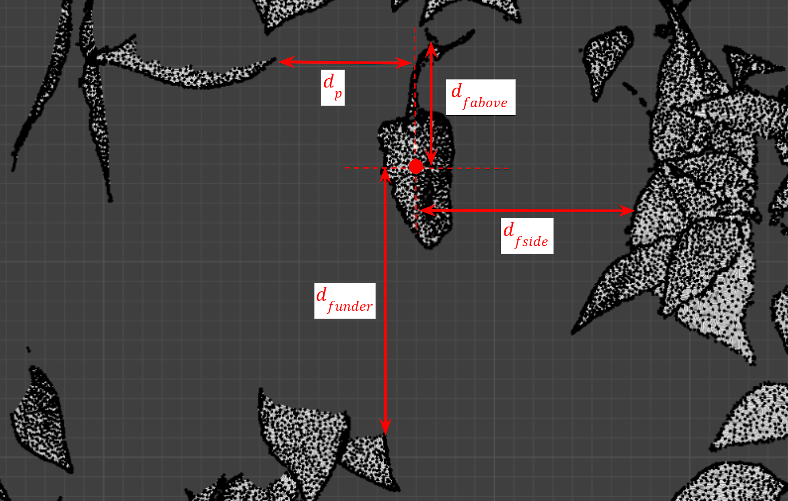
\includegraphics[width=\columnwidth]{images/png/measurement1.png}
     \caption{Measurement① distance to obstacle}
     \label{Fig:measurement1}
\end{figure}

\begin{figure}[H]
  \begin{minipage}[b]{0.48\columnwidth}
    \centering
    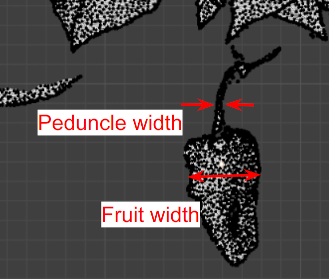
\includegraphics[width=\columnwidth]{images/png/measurement2.png}
    \caption{Measurement② width}
    \label{Fig:measurement2}
  \end{minipage}
  \hspace{0.04\columnwidth}
  \begin{minipage}[b]{0.48\columnwidth}
    \centering
    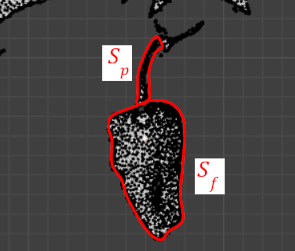
\includegraphics[width=\columnwidth]{images/png/measurement3.png}
    \caption{Measurement③ projection area}
    \label{Fig:measurement3}
  \end{minipage}
\end{figure}